\documentclass[]{beamer}
\setbeamertemplate{caption}[numbered]	% For numbered figures

\mode<presentation>
% Setup appearance:

\usetheme[secheader]{Boadilla}	% Standard theme for UIUC package
%\usetheme{Darmstadt}	%My standard for HEP
%\usetheme{Madrid}	%For information titles at bottom of screen
\usefonttheme[onlylarge]{structurebold}
\setbeamerfont*{frametitle}{size=\normalsize,series=\bfseries}
%\setbeamertemplate{navigation symbols}{}	% Suppresses all navigation symbols
\logo{
\includegraphics[height=1.0cm]{SMU_Logo_Red.pdf}}	%Inserts a logo in the lower right corner of the screen	%Comment out for faster compile
\setbeamercovered{transparent}


% Standard packages

\usepackage[english]{babel}

\usepackage{ifxetex}
\ifxetex
	%\usepackage{fontspec}
\else
	\usepackage[T1]{fontenc}
	\usepackage[latin1]{inputenc}
	\usepackage{lmodern}
\fi

\usepackage{times}
\usepackage{amsmath}  		% For math
\usepackage{amssymb}  		% For more math
\usepackage{mathrsfs}			%Fancy math, needed for Lagrangian scripts
\usepackage[normalem]{ulem} % For strikethrough
\usepackage{verbatim}		% For verbatim comments	Note: Must Declare the frame fragile first. \begin{frame}[fragile]
%\usepackage{multimedia}	% For movies
\usepackage{media9}		%Alternative movie package
\usepackage{calligra}		% For generating 'script r'
\DeclareMathAlphabet{\mathcalligra}{T1}{calligra}{m}{n}
\DeclareFontShape{T1}{calligra}{m}{n}{<->s*[2.2]callig15}{}

% A note about minted: You must compile from the command line as:
% pdflatex -shell-escape <file name here>
%\usepackage{minted}			% Provides syntax highlighting

% Custom Packages
\usepackage{custom}			% For custom math commands
\usepackage{InfolinesThemeJJ}	% Modified infolines outertheme; Modified by Juan Jottar UIUC 2010
\usepackage{JJmath}			% Custom math commands; Created by Juan Jottar UIUC 2010
\usepackage{beamercolorthemeSMU}		% Modified color palette to generate SMU colors 
% Additional packages for uiuc_beamer:
\usepackage{dsfont}
\usepackage{pstricks}
\usepackage{pst-node}
\usepackage{slashed}
\usepackage{graphicx} 	% For images
\graphicspath{{Images/}}

%\usepackage{mathtools}


% Setup TikZ

\usepackage{tikz}% 
\usetikzlibrary{fit}
\usetikzlibrary{calc}
%\usetikzlibrary{arrows}
%\tikzstyle{block}=[draw opacity=0.7,line width=1.4cm]


% Author, Title, etc.

\title[\LaTeX~Workshop for UT Austin SEG] 
{%
\LaTeX~Workshop for UT Austin\\ Geophysical Society%
}

\author[Matthew Feickert]			% For Sekula Group meetings
%\author[S. Sekula, M. Feickert]	% For meetings outside of SMU
{
 % Stephen~Sekula\inst{1} \and
  \textcolor{blue!50!black}{\href{http://www.matthewfeickert.com/}{Matthew~Feickert}}\inst{1}\\ \vspace{0.25cm}\href{https://twitter.com/HEPfeickert}{@HEPfeickert}
}

\institute[SMU Physics]
{
  \inst{1}%
  \href{http://www.physics.smu.edu/web/}{Southern Methodist University}
}

\date[March 12th, 2015]
{March 12th, 2015}

\AtBeginSection[]
{
  \begin{frame}<beamer>{Outline}
    \tableofcontents[currentsection]
  \end{frame}
}

% The main document

\begin{document}
%%%%%%%%%%%%%%%%%%%%%%%%%%%%%%%%%%%%%%%%%%%
\begin{frame}
  \titlepage
\end{frame}
%%%%%%%%%%%%%%%%%%%%%%%%%%%%%%%%%%%%%%%%%%%

%%%%%%%%%%%%%%%%%%%%%%%%%%%%%%
\section{Introduction to \LaTeX}
%%%%%%%%%%%%%%%%%%%%%%%%%%%%%%

\subsection*{Introduction}
%%%%%%%%%%%%%%%%%%%%%%%%%%%%%%

%%%%%%%%%%%%%%%%%%%%%%%%%%%%%%%%%%%%%%%%%%%
\begin{frame}{What is \LaTeX?}
\LaTeX~is a markup language written for the \TeX~typesetting program.
\begin{columns}[c]
\column{2.50in}
  \begin{block}{Features of \LaTeX}
    \begin{itemize}
    			\item Open source
    			\item Allows public to produce high-quality documents individually
			\item Provides identical output on all computers (both now and in the future)
			\item Widely used in academia
				\begin{itemize}
					\item Ex. Mathematics, computer science, economics, engineering, physics, and statistics.
				\end{itemize}
    \end{itemize}
  \end{block}
  %
\column{1.50in}
%%%%%%%%%%%%%%%%%   FIGURE   %%%%%%%%%%%%%%%%%
\begin{figure}[h!]
\centering
%
\includegraphics[scale=0.35]{CTAN_Lion.pdf}

\includegraphics[width=\textwidth]{CTAN_Lion.pdf}
\caption{\href{http://www.ctan.org/lion/}{CTAN} lion drawing by Duane Bibby.}
%\label{fig:}
\end{figure}
%%%%%%%%%%%%%%%%%%%%%%%%%%%%%%%%%%%%%%%%
  \end{columns}
\end{frame}

\subsection*{Why \LaTeX{}?}
%%%%%%%%%%%%%%%%%%%%%%%%%%%%%%

%%%%%%%%%%%%%%%%%%%%%%%%%%%%%%%%%%%%%%%%%%%
\begin{frame}{Why would I want to use \LaTeX{}?}
\textbf{Q.} Why would I want to learn how to use \LaTeX{} when I can just use Word?
	\begin{block}{Answer(s)}
		\begin{itemize}
			\item Open source
			\item Output is in PDF (through \href{http://en.wikipedia.org/wiki/PdfTeX}{pdf\TeX})
				\begin{itemize}
					\item Can view on any computer and never have to worry about presentation not showing up right.
				\end{itemize}
			%
			\item Ability to typeset mathematical equations quickly and cleanly
			\item Professional standard in academia
		\end{itemize}
	\end{block}
\end{frame}

%%%%%%%%%%%%%%%%%%%%%%%%%%%%%%%%%%%%%%%%%%%
\begin{frame}{Aren't these really just cosmetic reasons?}
Yes, but to some degree you will be judged by the quality of the way your present your work. Also, ease of dissemination of information is very important in research.
	\begin{block}{Bottom line}
%%%%%%%%%%%%%%%%%   FIGURE   %%%%%%%%%%%%%%%%%
\begin{figure}[h!tbp]
\centering
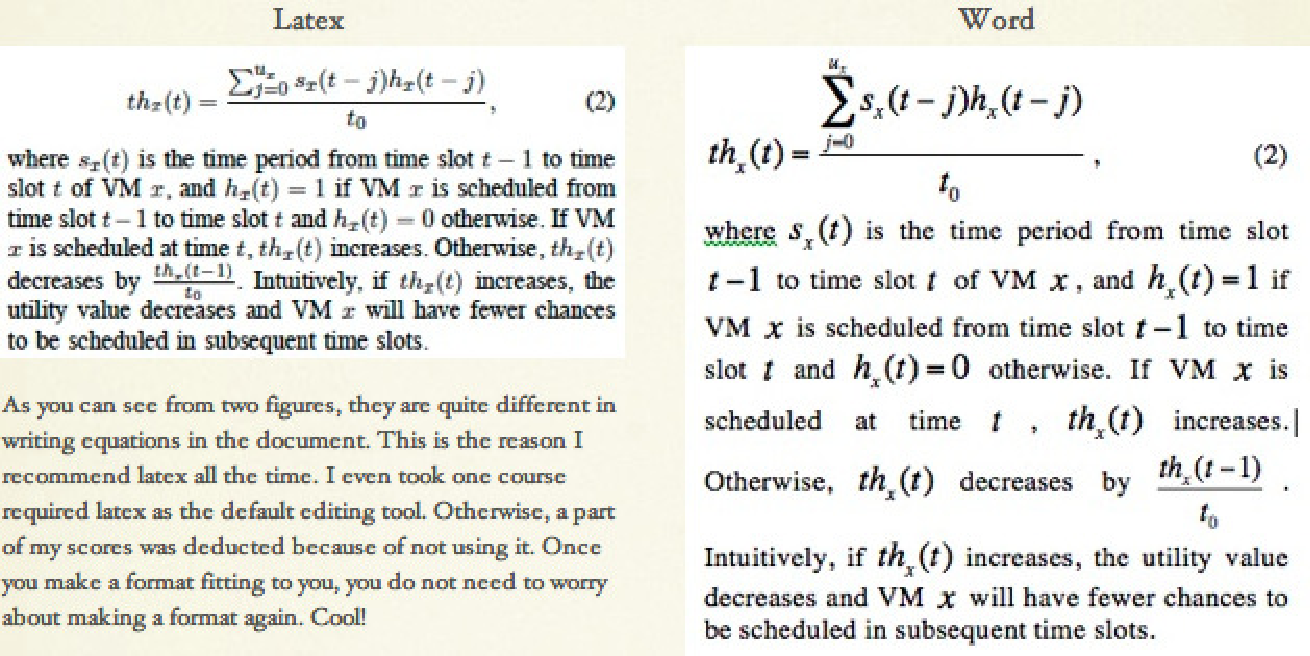
\includegraphics[scale=0.30]{latex_word_compare.pdf}
\caption{Credit: \href{http://home.gwu.edu/~jinho10/CS_Tips/Entries/2012/1/2_Latex_Tips.html}{\tiny http://home.gwu.edu/~jinho10/Home.html}}
%\label{fig:}
\end{figure}
%%%%%%%%%%%%%%%%%%%%%%%%%%%%%%%%%%%%%%%%
	\end{block}
\ldots which would you rather read?
\end{frame}


%%%%%%%%%%%%%%%%%%%%%%%%%%%%%%
\section{Setting Up \LaTeX~On Your Computer}
%%%%%%%%%%%%%%%%%%%%%%%%%%%%%%

%%%%%%%%%%%%%%%%%%%%%%%%%%%%%%%%%%%%%%%%%%%
\begin{frame}{Setup and Installation}
	\begin{block}{To get a \LaTeX~distribution on your computer}
		\begin{itemize}
    			\item Download and install the \href{http://www.latex-project.org/ftp.html}{distribution} for your operating system.
				\begin{itemize} \item Probably the latest version of \href{http://www.tug.org/texlive/}{\TeX~Live}.\end{itemize}
			\item Download and install a front end (or be hardcore and just use vim/emacs. :P)
				\begin{itemize}
					\item Windows: \href{http://miktex.org/}{MiKTeX}
					\item Mac: \href{http://pages.uoregon.edu/koch/texshop/}{TeXShop}
					\item Linux: \href{http://www.tug.org/texworks/}{TeXworks}
				\end{itemize}
			%
			\item Install any packages you want in the proper directory
			\item Start creating!
    		\end{itemize}
	\end{block}
\end{frame}
%%%%%%%%%%%%%%%%%%%%%%%%%%%%%%
\section{Creating a \LaTeX~Document}
%%%%%%%%%%%%%%%%%%%%%%%%%%%%%%

\subsection*{A simple document}
%%%%%%%%%%%%%%%%%%%%%%%%%%%%%%

%%%%%%%%%%%%%%%%%%%%%%%%%%%%%%%%%%%%%%%%%%%
\begin{frame}[fragile]{Open The (Web) Editor: Overleaf}
For today's workshop we're going to be using a web front end: \textcolor{green!80!black}{Overleaf}
\begin{enumerate}
	\item Navigate to \href{https://www.overleaf.com/}{www.overleaf.com}
	\item Click the \href{https://www.overleaf.com/docs?template=overleaf}{``Create A New Paper'' button}
\begin{figure}[!htbp]
\centering

\includegraphics[scale=0.40]{Overleaf_Create_Paper.png}
\end{figure}
%%%%%%%%%%%%%%%%%%%%%%%%%%%%%%%%%%%%%%%%
		\item Once the template is loaded, click the ``Source'' button in the upper left corner
		\item We're going to start from scratch, so select all and delete
\end{enumerate}
\end{frame}

%%%%%%%%%%%%%%%%%%%%%%%%%%%%%%%%%%%%%%%%%%%
\begin{frame}[fragile]{Creating a (simple) document}
\begin{verbatim}
\documentclass{article}

\begin{document}

Hello, World!

\end{document}
\end{verbatim}
\end{frame}

%%%%%%%%%%%%%%%%%%%%%%%%%%%%%%%%%%%%%%%%%%%
\begin{frame}[fragile]{Creating a (simple) document}
\begin{verbatim}
\documentclass{article}

\begin{document}

Hello, World!\\

The quick brown fox jumps over the lazy dog.

\end{document}
\end{verbatim}
\end{frame}

\subsection*{Expanding: The Preamble}
%%%%%%%%%%%%%%%%%%%%%%%%%%%%%%

%%%%%%%%%%%%%%%%%%%%%%%%%%%%%%%%%%%%%%%%%%%
\begin{frame}[fragile]{Creating a document}
\small\begin{verbatim}
\documentclass[letterpaper,12pt]{article}

\usepackage{graphicx} % For images
\usepackage{float}			   % For tables and other floats
\usepackage{amsmath} 	% For math
\usepackage{amssymb}				 % For more math
\usepackage{fullpage} % Set margins & place page numbers
\usepackage{mathrsfs}		% For nice math calligraphy fonts
\usepackage{verbatim}		% Allows commenting out
\begin{document}

Hello, World!\\
$\sin x \cdot \tan x \times \alpha \beta$\\
$\gamma \sum \prod \sqrt{y}$

\end{document}
\end{verbatim}
\end{frame}

%%%%%%%%%%%%%%%%%%%%%%%%%%%%%%%%%%%%%%%%%%%
\begin{frame}[fragile]{Creating a paper}
\small\begin{verbatim}
\documentclass[letterpaper,12pt]{article}

\title{The Title of a Paper of Great Importance}
\author{First Author}

\begin{document}
\maketitle

\begin{abstract}
Here is a collection of words that form a run on sentence 
to test an idea that was formed in a brain made of cells 
made of molecules made of atoms made of patrons and 
leptons and nope screw string theory.
\end{abstract}
\clearpage
Stuff and things go here
\end{document}
\end{verbatim}
\end{frame}

\subsection*{Figure Basics}
%%%%%%%%%%%%%%%%%%%%%%%%%%%%%%
%%%%%%%%%%%%%%%%%%%%%%%%%%%%%%%%%%%%%%%%%%%
\begin{frame}[fragile]{Inserting Figures}
\small\begin{verbatim}
\documentclass[letterpaper,12pt]{article}
...
\usepackage{graphicx}
%\graphicspath{{Images/}} %Overleaf has frog.jpg in the 
						  %local dir but in general set 
						  %to your dir with figures 
...
\begin{document}
...
\begin{figure}
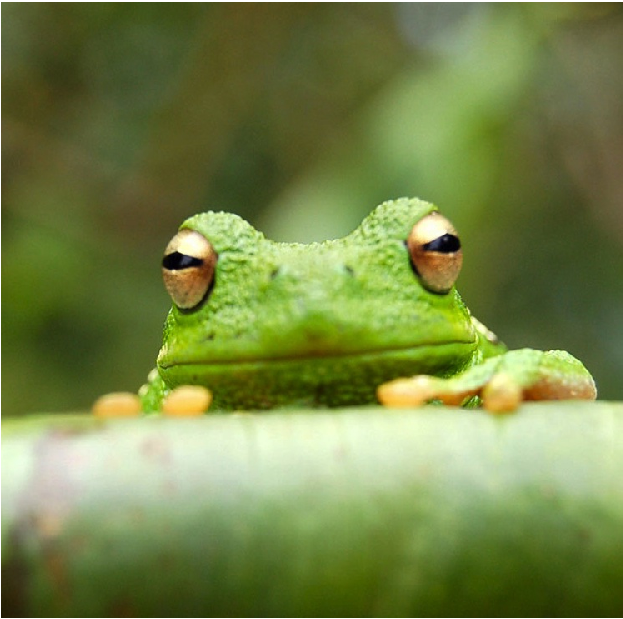
\includegraphics[width=\textwidth]{frog.jpg}
\end{figure}
...
\end{document}
\end{verbatim}
\end{frame}

%%%%%%%%%%%%%%%%%%%%%%%%%%%%%%%%%%%%%%%%%%%
\begin{frame}[fragile]{Inserting Figures}
\begin{figure}
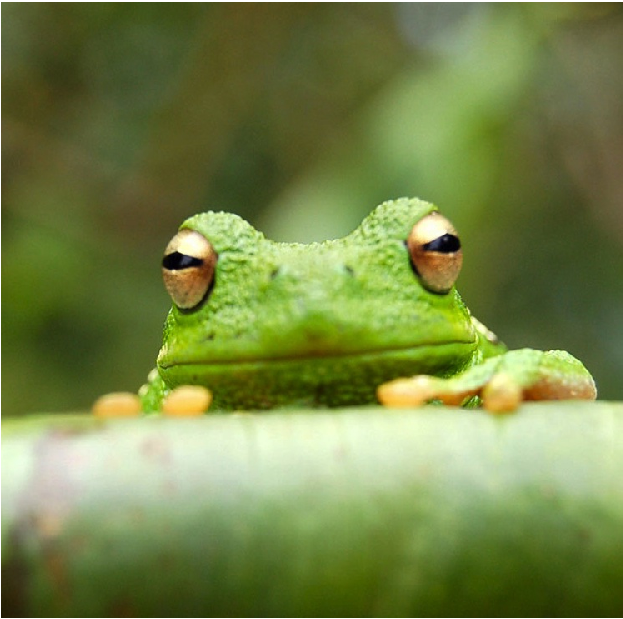
\includegraphics[width=0.50\textwidth]{frog.pdf}
%\label{Fig:frogA}
\end{figure}
\end{frame}
%%%%%%%%%%%%%%%%%%%%%%%%%%%%%%%%%%%%%%%%

%%%%%%%%%%%%%%%%%%%%%%%%%%%%%%%%%%%%%%%%%%%
\begin{frame}[fragile]{Better Figures}
\small\begin{verbatim}
\documentclass[letterpaper,12pt]{article}
...
\usepackage{graphicx}
%\graphicspath{{Images/}}
...
\begin{document}
...
\begin{figure}[!htbp]  %here, top, bottom, page.
\centering
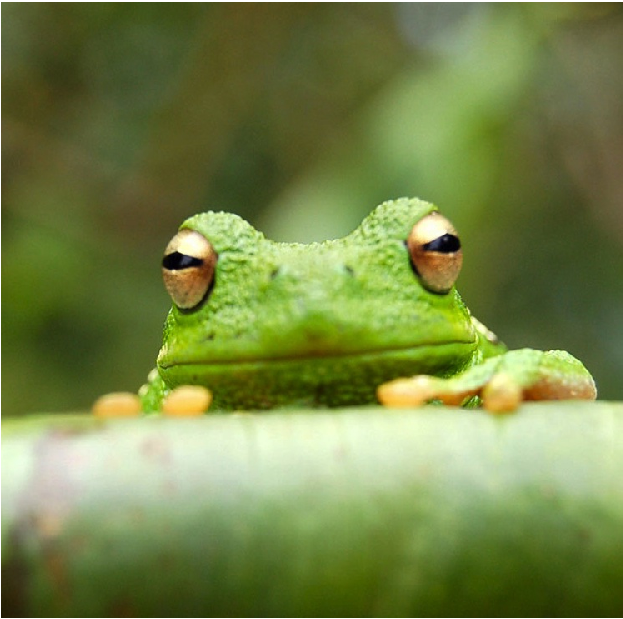
\includegraphics[width=\textwidth]{frog.jpg}
\caption{This is a frog!}
\label{Fig:frog}
\end{figure}
...
\end{document}
\end{verbatim}
\end{frame}
%%%%%%%%%%%%%%%%%%%%%%%%%%%%%%%%%%%%%%%%

%%%%%%%%%%%%%%%%%%%%%%%%%%%%%%%%%%%%%%%%%%%
\begin{frame}[fragile]{Better Figures}
\begin{figure}[!htbp]
\centering
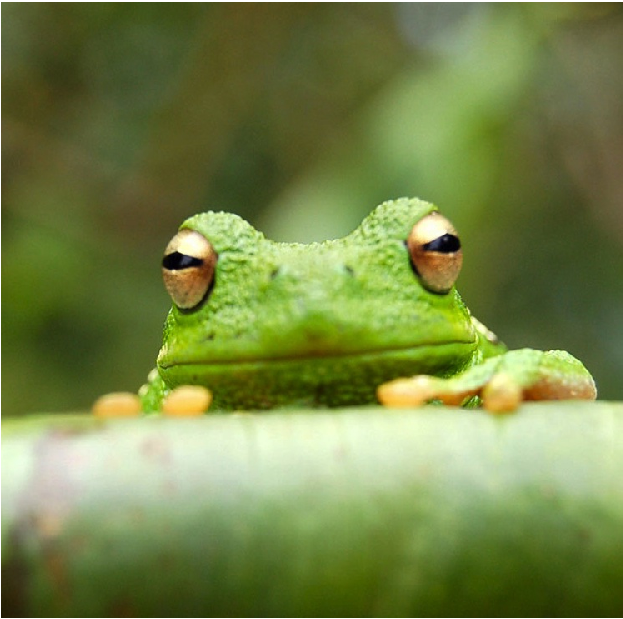
\includegraphics[width=0.50\textwidth]{frog.pdf}
\caption{This is a frog!}
\label{Fig:frogB}
\end{figure}
\end{frame}
%%%%%%%%%%%%%%%%%%%%%%%%%%%%%%%%%%%%%%%%

%%%%%%%%%%%%%%%%%%%%%%%%%%%%%%%%%%%%%%%%%%%
\begin{frame}[fragile]{Rescaling Figures}
\small\begin{verbatim}
\documentclass[letterpaper,12pt]{article}
...
\usepackage{graphicx}
%\graphicspath{{Images/}}
...
\begin{document}
...
\begin{figure}[h!tbp]
\centering
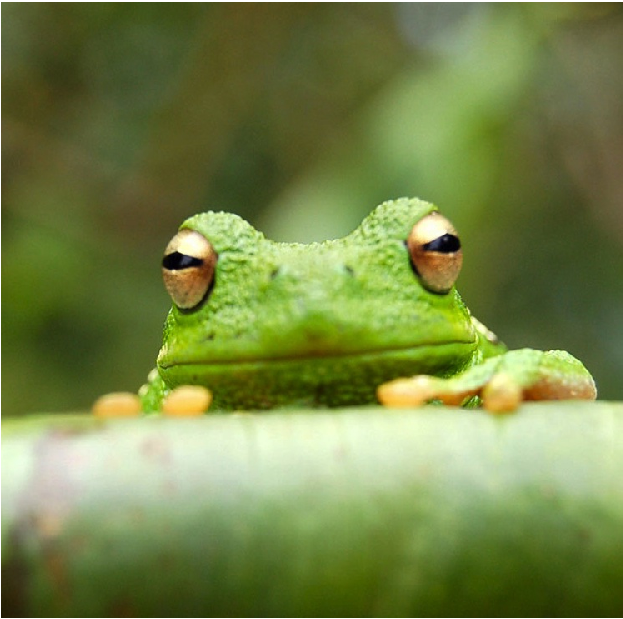
\includegraphics[scale=0.40]{frog.jpg}
\caption{This is a frog!}
\label{Fig:frog}
\end{figure}
...
\end{document}
\end{verbatim}
\end{frame}
%%%%%%%%%%%%%%%%%%%%%%%%%%%%%%%%%%%%%%%%

%%%%%%%%%%%%%%%%%%%%%%%%%%%%%%%%%%%%%%%%%%%
\begin{frame}[fragile]{Rescaling Figures}
\begin{figure}[h!tbp]
\centering
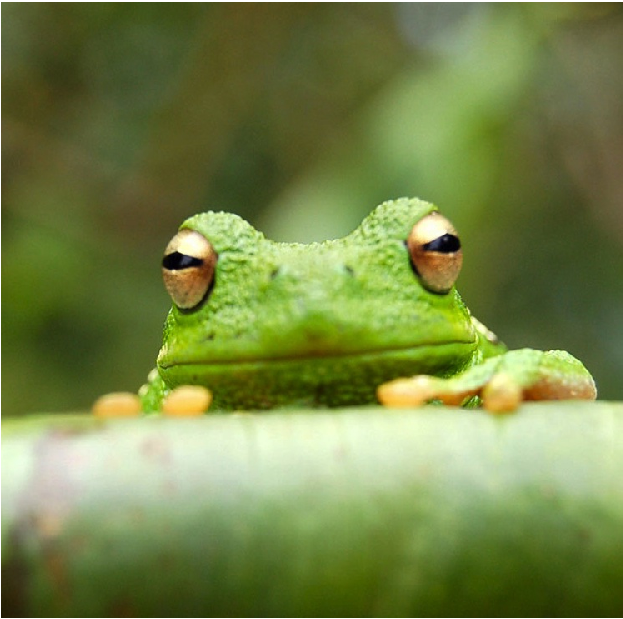
\includegraphics[scale=0.40]{frog.pdf}
\caption{This is a frog!}
\label{Fig:frogC}
\end{figure}
\end{frame}
%%%%%%%%%%%%%%%%%%%%%%%%%%%%%%%%%%%%%%%%

%%%%%%%%%%%%%%%%%%%%%%%%%%%%%%%%%%%%%%%%%%%
\begin{frame}[fragile]{Rescaling Figures}
\small\begin{verbatim}
\documentclass[letterpaper,12pt]{article}
...
\usepackage{graphicx}
%\graphicspath{{Images/}}
...
\begin{document}
...
\begin{figure}[h!tbp]
\centering
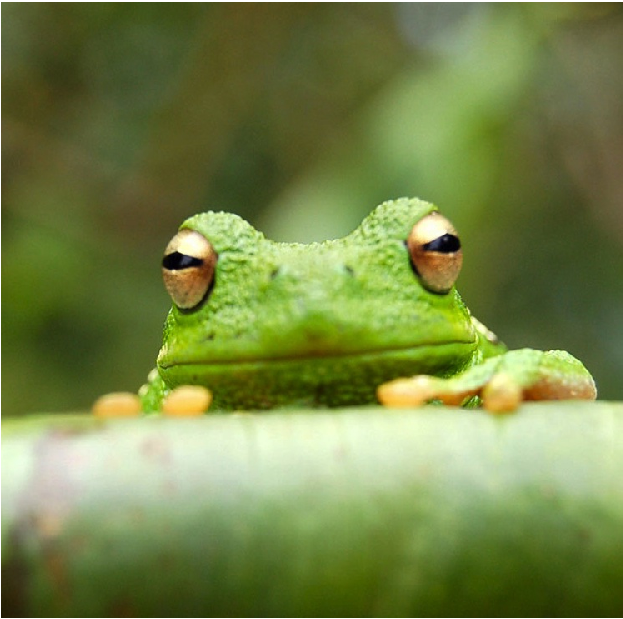
\includegraphics[width=0.80\textwidth]{frog.jpg}
\caption{This is a frog!}
\label{Fig:frog}
\end{figure}
...
\end{document}
\end{verbatim}
\end{frame}
%%%%%%%%%%%%%%%%%%%%%%%%%%%%%%%%%%%%%%%%

%%%%%%%%%%%%%%%%%%%%%%%%%%%%%%%%%%%%%%%%%%%
\begin{frame}[fragile]{Rescaling Figures}
\begin{figure}[h!tbp]
\centering
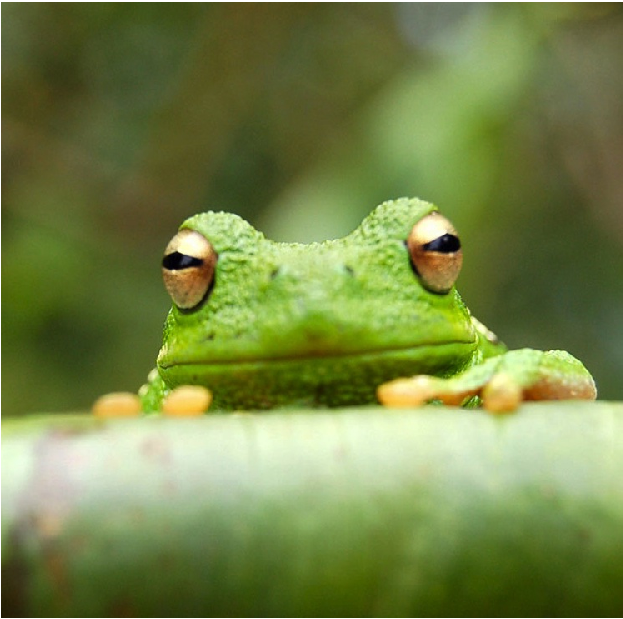
\includegraphics[width=0.35\textwidth]{frog.pdf}
\caption{This is a frog!}
\label{Fig:frogD}
\end{figure}
\end{frame}
%%%%%%%%%%%%%%%%%%%%%%%%%%%%%%%%%%%%%%%%

%%%%%%%%%%%%%%%%%%%%%%%%%%%%%%
\section{Math Mode}
%%%%%%%%%%%%%%%%%%%%%%%%%%%%%%

%%%%%%%%%%%%%%%%%%%%%%%%%%%%%%%%%%%%%%%%%%%
\begin{frame}{Typesetting in Math Mode}
Typesetting in Math Mode is what really gives \LaTeX{} its power. It is intuitive, quick, clean, and produces wonderful results! To initiate Math Mode enclose whatever you want to typeset between two ``\$''.
	\begin{block}{Some examples}
		\begin{itemize}
    			\item \$\textbackslash Sigma\$ = $\Sigma$
			\item \$\textbackslash int f(x) \textbackslash,dx\$ = $\int f(x)\,dx$
			\item \$e\textasciicircum x\_\{\textbackslash text\{text\}\}\$ = $e^x_{\text{text}}$
			\item \$\textbackslash frac\{\textbackslash sin x\}\{\textbackslash prod\_\{i=0\}\textasciicircum n\}\$ = $\frac{\sin x}{\prod_{i=0}^n}$
    		\end{itemize}
	\end{block}
and so\ldots
\[
\imply \int\limits_{\rho}^R \frac{\sqrt[3]{r}\,\ln r}{r^2 + 1}~dr + \int_{L_2} f(z)~dz = e^{i \pi/3} \int\limits_{\rho}^R \frac{\sqrt[3]{r}\,\ln r + i \pi \sqrt[3]{r}}{r^2 + 1}~dr% = \frac{i\pi^2}{2}\,e^{i \pi/6} - \int_{C_\rho} f(z)~dz - \int_{C_R} f(z)~dz
\]
\end{frame}

%%%%%
\begin{frame}{Math Mode: Display Style}
The displaymath environment will pop your equation out of the text and display it prominently in the center of the page.
	\begin{block}{In Line vs. Displayed}
		\begin{itemize}
    			\item It is seen that this requires $C = -k^2$, where $k^2>0$, reducing to $\rho\partiald{}{\rho} \parenthsqr{\rho \partiald{R\parenth{\rho}}{\rho}} - \parenth{n^2 - \rho^2 k^2} R\parenth{\rho} = 0.$
			\item It is seen that this requires $C = -k^2$, where $k^2>0$, reducing to \[\rho\partiald{}{\rho} \parenthsqr{\rho \partiald{R\parenth{\rho}}{\rho}} - \parenth{n^2 - \rho^2 k^2} R\parenth{\rho} = 0.\]
    		\end{itemize}
	\end{block}
\end{frame}

%%%%%
\begin{frame}{Math Mode: Display Style}
The displaymath environment is entered by enclosing whatever you want to typeset between opening ``\textbackslash['' and closing ``\textbackslash]''.
	\begin{block}{In Line vs. Displayed}
		\begin{itemize}
    			\item \$\textbackslash int \textbackslash limits\_\{-\textbackslash infty\}\textasciicircum \{\textbackslash infty\} \textbackslash psi\textasciicircum* \textbackslash psi \textbackslash,dx \$ = $\infint \psi^* \psi\,dx$
			\item \textbackslash[ \textbackslash int \textbackslash limits\_\{-\textbackslash infty\}\textasciicircum \{\textbackslash infty\} \textbackslash psi\textasciicircum* \textbackslash psi \textbackslash,dx \textbackslash] = \[\infint \psi^* \psi\,dx \]
    		\end{itemize}
	\end{block}
\end{frame}

%%%%%%%%%%%%%%%%%%%%%%%%%%%%%%
\section{Packages \& Fun!}
%%%%%%%%%%%%%%%%%%%%%%%%%%%%%%

%%%%%%%%%%%%%%%%%%%%%%%%%%%%%%%%%%%%%%%%%%%
\begin{frame}{Fun with Packages!}
There are a ton of really useful packages, and just fun packages that you can use to make your documents stand out and entertaining.
	\begin{block}{One useful and N fun packages}
		\begin{itemize}
    			\item My ``\href{http://dl.dropbox.com/u/6351966/custom.sty}{custom}'' style file (what I use for \TeX ing~my homework).
			\item \href{http://hanno-rein.de/archives/349}{Coffee stains}
			\item \href{http://tug.ctan.org/tex-archive/usergrps/uktug/baskervi/4_4/}{The Simpsons}
    		\end{itemize}
	\end{block}
\end{frame}

%%%%%%%%%%%%%%%%%%%%%%%%%%%%%%
\section{Summary}
%%%%%%%%%%%%%%%%%%%%%%%%%%%%%%

%%%%%
\begin{frame}{What Can I Do With \LaTeX?}
\begin{block}{``Fancy'' looking equations}
The Lagrangian for the ABC ``toy'' theory containing three elementary particles of spin 0, masses $m_{A,B,C}$, and one primitive vertex with the vertex factor $-ig$.
\[
\begin{split}
\Lagrangian	&= \parenthsqr{\frac{1}{2} \parenth{\partial_\mu \phi_A} \parenth{\partial^\mu \phi_A} - \frac{1}{2} \parenth{\frac{m_A c}{\hbar}}^2 \phi_A^2}	\\
	&+ \parenthsqr{\frac{1}{2} \parenth{\partial_\mu \phi_B} \parenth{\partial^\mu \phi_B} - \frac{1}{2} \parenth{\frac{m_B c}{\hbar}}^2 \phi_B^2}\\
&+ \parenthsqr{\frac{1}{2} \parenth{\partial_\mu \phi_C} \parenth{\partial^\mu \phi_C} - \frac{1}{2} \parenth{\frac{m_C c}{\hbar}}^2 \phi_C^2} - g \phi_A \phi_B \phi_C
\end{split}
\]
\end{block}
\end{frame}

%%%%%
\begin{frame}{What Can I Do With \LaTeX?}
\begin{block}{Homework\ldots with fancy looking equations}
\begin{figure}[h!tbp]
\centering
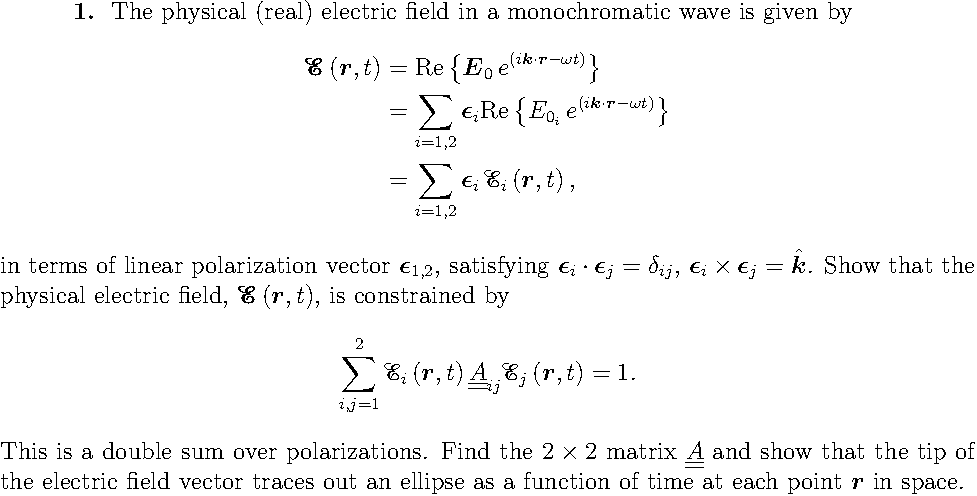
\includegraphics[width=\textwidth]{Homework_Example.pdf}
%caption{}
%label{fig:}
\end{figure}
%%%%%%%%%%%%%%%%%%%%%%%%%%%%%%%%%%%%%%%%
\end{block}
\end{frame}


%%%%%
\begin{frame}{What Can I Do With \LaTeX?}
	\begin{block}{Draw All The Things (with \href{http://en.wikipedia.org/wiki/PGF/TikZ}{TikZ})}
%%%%%%%%%%%%%%%%%   TIKZ FIGURE   %%%%%%%%%%%%%%%%%
\begin{figure}[h!tbp]
\centering
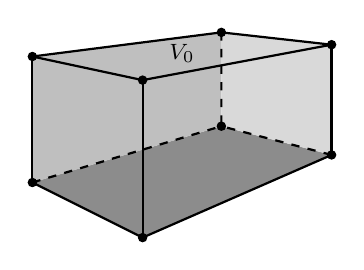
\begin{tikzpicture}
	%%% Edit the following coordinate to change the shape of your
	%%% cuboid
      
	%% Vanishing points for perspective handling
	\coordinate (P1) at (-7cm,1.5cm); % left vanishing point (To pick)
	\coordinate (P2) at (8cm,1.5cm); % right vanishing point (To pick)

	%% (A1) and (A2) defines the 2 central points of the cuboid
	\coordinate (A1) at (0em,0cm); % central top point (To pick)
	\coordinate (A2) at (0em,-2cm); % central bottom point (To pick)

	%% (A3) to (A8) are computed given a unique parameter (or 2) .8
	% You can vary .8 from 0 to 1 to change perspective on left side
	\coordinate (A3) at ($(P1)!.8!(A2)$); % To pick for perspective 
	\coordinate (A4) at ($(P1)!.8!(A1)$);

	% You can vary .8 from 0 to 1 to change perspective on right side
	\coordinate (A7) at ($(P2)!.7!(A2)$);
	\coordinate (A8) at ($(P2)!.7!(A1)$);

	%% Automatically compute the last 2 points with intersections
	\coordinate (A5) at
	  (intersection cs: first line={(A8) -- (P1)},
			    second line={(A4) -- (P2)});
	\coordinate (A6) at
	  (intersection cs: first line={(A7) -- (P1)}, 
			    second line={(A3) -- (P2)});

	%%% Depending of what you want to display, you can comment/edit
	%%% the following lines
	
		%% Possibly draw front faces
		% \fill[orange] (A1) -- (A8) -- (A7) -- (A2) -- cycle; % face 1
	% \node at (barycentric cs:A1=1,A8=1,A7=1,A2=1) {\tiny f1};
	\fill[gray!50,opacity=0.2] (A1) -- (A2) -- (A3) -- (A4) -- cycle; % f2
	%\node at (barycentric cs:A1=1,A2=1,A3=1,A4=1) {\tiny f2};
	\fill[gray!90,opacity=0.2] (A1) -- (A4) -- (A5) -- (A8) -- cycle; % f5

	%% Possibly draw back faces

	\fill[gray!90] (A2) -- (A3) -- (A6) -- (A7) -- cycle; % face 6
	%\node at (barycentric cs:A2=1,A3=1,A6=1,A7=1) {\tiny f6};
	
	\fill[gray!50] (A3) -- (A4) -- (A5) -- (A6) -- cycle; % face 3
	%\node at (barycentric cs:A3=1,A4=1,A5=1,A6=1) {\tiny f3};
	
	\fill[gray!30] (A5) -- (A6) -- (A7) -- (A8) -- cycle; % face 4
	%\node at (barycentric cs:A5=1,A6=1,A7=1,A8=1) {\tiny f4};
	
	\draw[thick,dashed] (A5) -- (A6);
	\draw[thick,dashed] (A3) -- (A6);
	\draw[thick,dashed] (A7) -- (A6);

	%% Possibly draw front faces

	\node at (barycentric cs:A1=1,A4=1,A5=1,A8=1) {\footnotesize $V_0$};	%{\tiny f5};

	%% Possibly draw front lines
	\draw[thick] (A1) -- (A2);
	\draw[thick] (A3) -- (A4);
	\draw[thick] (A7) -- (A8);
	\draw[thick] (A1) -- (A4);
	\draw[thick] (A1) -- (A8);
	\draw[thick] (A2) -- (A3);
	\draw[thick] (A2) -- (A7);
	\draw[thick] (A4) -- (A5);
	\draw[thick] (A8) -- (A5);
	
	% Possibly draw points
	% (it can help you understand the cuboid structure)
	\foreach \i in {1,2,...,8}
	{
	  \draw[fill=black] (A\i) circle (0.15em);
	   % node[above right] {\tiny \i};
	}
	% \draw[fill=black] (P1) circle (0.1em) node[below] {\tiny p1};
	% \draw[fill=black] (P2) circle (0.1em) node[below] {\tiny p2};
\end{tikzpicture}
%\caption{}
\label{fig:}
\end{figure}
%%%%%%%%%%%%%%%%%%%%%%%%%%%%%%%%%%%%%%%%

%%%%%%%%%%%%%%%%%   TIKZ FIGURE   %%%%%%%%%%%%%%%%%
\begin{figure}[h!tbp]
\centering
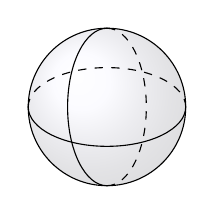
\begin{tikzpicture}
	\shade[ball color=blue!10!white,opacity=0.20] (0,0) circle (1cm);
    \draw (-1,0) arc (180:360:1cm and 0.5cm);
    \draw[dashed] (-1,0) arc (180:0:1cm and 0.5cm);
    \draw (0,1) arc (90:270:0.5cm and 1cm);
    \draw[dashed] (0,1) arc (90:-90:0.5cm and 1cm);
    \draw (0,0) circle (1cm);
%    \shade[ball color=blue!10!white,opacity=0.20] (0,0) circle (1cm);
\end{tikzpicture}
%\caption{}
%\label{fig:}
\end{figure}
%%%%%%%%%%%%%%%%%%%%%%%%%%%%%%%%%%%%%%%%
	\end{block}
\end{frame}

%%%%%%%%%%%%%%%%%%%%%%%%%%%%%%%%%%%%%%%%%%%
\begin{frame}{What Can I Do With \LaTeX?}
  \begin{block}{More Like ``What Can't You Do!?''}
    \begin{itemize}
    	\item Typeset professional documents
    		\begin{itemize}
			\item Ex. Thesis, \href{http://matthewfeickert.github.io/mfeickert-CV.pdf}{CV}, Reports
		\end{itemize}
	%
	\item Create presentations in pdf
		\begin{itemize}
			\item Ex. \href{https://github.com/matthewfeickert/UTAustin-LaTeX-Workshop-2015}{This presentation}! (You can even embed video using the \href{https://www.ctan.org/pkg/media9}{media9} package. 0\_0)
		\end{itemize}
	%
	\item Circuit diagrams (\href{http://www.ctan.org/tex-archive/graphics/pgf/contrib/circuitikz}{circuitikz} package)
	\item Feynman diagrams (\href{http://osksn2.hep.sci.osaka-u.ac.jp/~taku/osx/feynmp.html}{feynmp} package)
	\item \href{http://casa.colorado.edu/~danforth/comp/cardtex.html}{Business cards}
	\item Conference posters (\href{http://www-i6.informatik.rwth-aachen.de/~dreuw/latexbeamerposter.php}{beamerposter} package)
	\item \ldots basically everything!
    \end{itemize}
  \end{block}
\end{frame}

%#######################
%%%%%%%%%%%%%%%%
%   END MAIN PRESENTATION
%%%%%%%%%%%%%%%%
%#######################

%%%%%%%%%%%%%%%%%%%%%%%%%%%%%%%%%%%%%%%%%%%
\section*{Backup Slides}
%%%%%%%%%%%%%%%%%%%%%%%%%%%%%%%%%%%%%%%%%%%

%%%%%%%%%%%%%%%%%%%%%%%%%%%%%%%%%%%%%%%%%%%
\begin{frame}{Backup Slides}
  \begin{center}
{\alert{\Huge{Backup}}}
  \end{center}
\end{frame}

\subsection*{\LaTeX{} Resources}
%%%%%%%%%%%%%%%%%%%%%%%%%%%%%%
%%%%%%%%%%%%%%%%%%%%%%%%%%%%%%%%%%%%%%%%%%%
\begin{frame}{How Can I Learn More About \LaTeX{}?}
	\begin{itemize}
		\item \href{https://www.ctan.org/}{Comprehensive \TeX{} Archive Network (CTAN)}
		\item There are lots of great online resources. A great place to start is \href{https://www.overleaf.com/}{Overleaf}.
			\begin{itemize}
				\item Free student accounts
				\item Free \href{https://www.overleaf.com/latex/learn/free-online-introduction-to-latex-part-1\#.VPkJ7c3d-oo}{\LaTeX{} tutorial} very similar to one given tonight
			\end{itemize}
		\item Questions or confused? Check the \href{http://tex.stackexchange.com/}{\TeX{} Stack Exchange}
		\item Ask people who have used \LaTeX{}. They're usually happy to share their tricks of the trade.
	\end{itemize}
\end{frame}

\subsection*{Packages}
%%%%%%%%%%%%%%%%%%%%%%%%%%%%%%

%%%%%%%%%%%%%%%%%%%%%%%%%%%%%%%%%%%%%%%%%%%
\begin{frame}{Installing packages}
	\begin{itemize}
		\item Most distributions will come with a package manager. It let's you search and install packages by query.
		\item If you don't know where to install a package so it can be universally accessed by your operating system, just save it in the same directory as your \TeX~file.
		\item If you're working on a Windows machine you'll probably need to run ``\href{http://tex.stackexchange.com/questions/48292/about-texhash-and-proper-installation-of-texlive}{texhash}'' from the command prompt before your computer will recognize the new package.
	\end{itemize}
\end{frame}

\subsection*{Macros}
%%%%%%%%%%%%%%%%%%%%%%%%%%%%%%

%%%%%%%%%%%%%%%%%%%%%%%%%%%%%%%%%%%%%%%%%%%
\begin{frame}[fragile]{Figure}
\begin{verbatim}
%%%%%%%%%%%%%%%%%   FIGURE   %%%%%%%%%%%%%%%%%
\begin{figure}[h!tbp]
\centering
\includegraphics[scale=1.00]{}
%\caption{}
%\label{fig:}
\end{figure}
%%%%%%%%%%%%%%%%%%%%%%%%%%%%%%%%%%%%%%%%
\end{verbatim}
\end{frame}

%%%%%%%%%%%%%%%%%%%%%%%%%%%%%%%%%%%%%%%%%%%
\begin{frame}[fragile]{Figure: Example}
\begin{verbatim}
%%%%%%%%%%%%%%%%%   FIGURE   %%%%%%%%%%%%%%%%%
\begin{figure}[h!tbp]
\centering
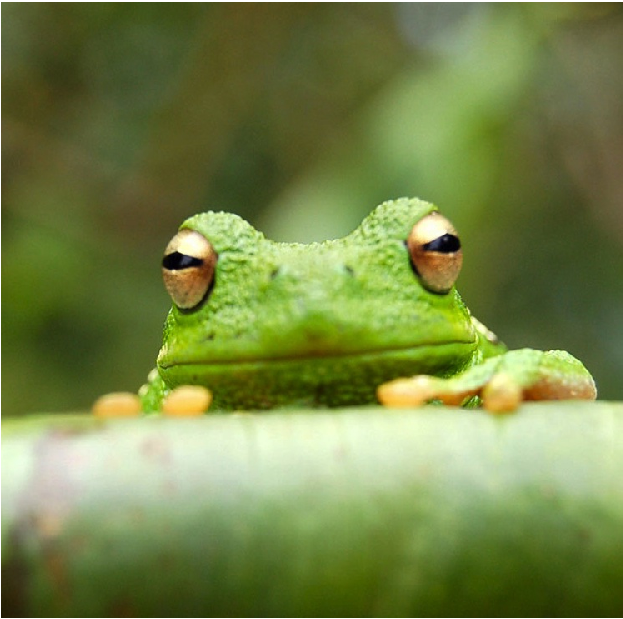
\includegraphics[scale=0.40]{frog.pdf}
\caption{Here is a very interesting picture of a frog.}
\label{fig:frog}
\end{figure}
%%%%%%%%%%%%%%%%%%%%%%%%%%%%%%%%%%%%%%%%

Noting Figure~\ref{fig:frog}, it is seen that\ldots
\end{verbatim}
\end{frame}

%%%%%%%%%%%%%%%%%%%%%%%%%%%%%%%%%%%%%%%%%%%
\begin{frame}{Figure: Example}
%%%%%%%%%%%%%%%%%   FIGURE   %%%%%%%%%%%%%%%%%
\begin{figure}[h!tbp]
\centering
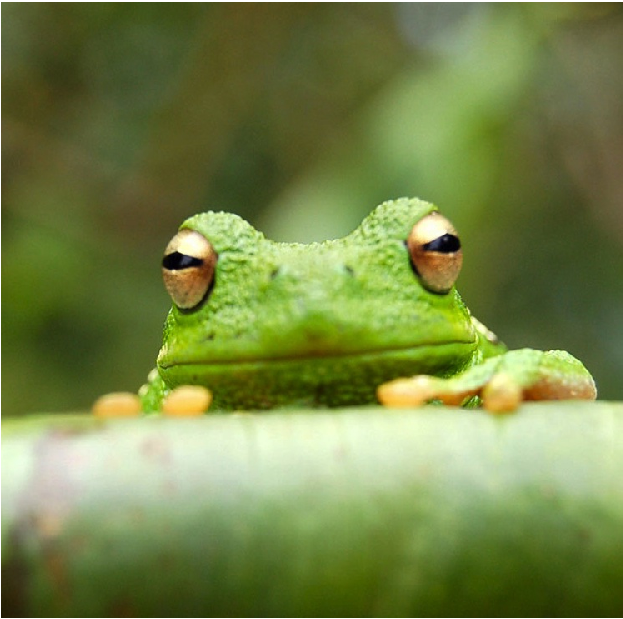
\includegraphics[scale=0.40]{frog.pdf}
\caption{Here is a very interesting picture of a frog.}
\label{fig:frog}
\end{figure}
%%%%%%%%%%%%%%%%%%%%%%%%%%%%%%%%%%%%%%%%

Noting Figure~\ref{fig:frog}, it is seen that\ldots
\end{frame}

%%%%%%%%%%%%%%%%%%%%%%%%%%%%%%%%%%%%%%%%%%%
\begin{frame}[fragile]{Table}
\begin{verbatim}
%%%%%%%%%%%%%%%%%   TABLE   %%%%%%%%%%%%%%%%%
\begin{table}[!hbtp]
\caption{Caption}
\centering
\scalebox{1.00}{
\begin{tabular}[!hbtp]{ | c | c | c | }
\hline\hline

\hline\hline
\end{tabular}}
\label{table:TABLE}
\end{table}
%%%%%%%%%%%%%%%%%%%%%%%%%%%%%%%%%%%%%%%%
\end{verbatim}
\end{frame}

%%%%%%%%%%%%%%%%%%%%%%%%%%%%%%%%%%%%%%%%%%%
\begin{frame}[fragile]{Equation}
\begin{verbatim}
%%%%%%%%%%%   EQUATION   %%%%%%%%%%%
\begin{equation}

\label{eq:1}
\end{equation}
%%%%%%%%%%%%%%%%%%%%%%%%%%%%%%
\end{verbatim}
\end{frame}

%%%%%%%%%%%%%%%%%%%%%%%%%%%%%%%%%%%%%%%%%%%
\begin{frame}[fragile]{Equation: Example}
\begin{verbatim}
%%%%%%%%%%%   EQUATION   %%%%%%%%%%%
\begin{equation}
\alpha + \beta = \gamma
\label{eq:alpha}
\end{equation}
%%%%%%%%%%%%%%%%%%%%%%%%%%%%%%

Here is Equation~\ref{eq:alpha}.
\end{verbatim}
\end{frame}

%%%%%%%%%%%%%%%%%%%%%%%%%%%%%%%%%%%%%%%%%%%
\begin{frame}{Equation: Example}
%%%%%%%%%%%   EQUATION   %%%%%%%%%%%
\begin{equation}
\alpha + \beta = \gamma
\label{eq:alpha}
\end{equation}
%%%%%%%%%%%%%%%%%%%%%%%%%%%%%%

Here is Equation~\ref{eq:alpha}.
\end{frame}

%%%%%%%%%%%%%%%%%%%%%%%%%%%%%%%%%%%%%%%%%%%
\begin{frame}[fragile]{Matrix}
\begin{verbatim}
%%%%%%%%%%%  MATRIX   %%%%%%%%%%%
\begin{pmatrix}
X & X\\
\end{pmatrix}
%%%%%%%%%%%%%%%%%%%%%%%%%%%%%%
\end{verbatim}
\end{frame}

%%%%%%%%%%%%%%%%%%%%%%%%%%%%%%%%%%%%%%%%%%%
\begin{frame}[fragile]{Matrix: Example}
\begin{verbatim}
%%%%%%%%%%%  MATRIX   %%%%%%%%%%%
\[
\begin{pmatrix}
1 & 0\\
0 & 1
\end{pmatrix}
\]
%%%%%%%%%%%%%%%%%%%%%%%%%%%%%%
\end{verbatim}
\end{frame}

%%%%%%%%%%%%%%%%%%%%%%%%%%%%%%%%%%%%%%%%%%%
\begin{frame}{Matrix: Example}
%%%%%%%%%%%  MATRIX   %%%%%%%%%%%
\[
\begin{pmatrix}
1 & 0\\
0 & 1
\end{pmatrix}
\]
%%%%%%%%%%%%%%%%%%%%%%%%%%%%%%
\end{frame}

%%%%%%%%%%%%%%%%%%%%%%%%%%%%%%%%%%%%%%%%%%%
\begin{frame}[fragile]{Split line equation}
\begin{verbatim}
\[
\begin{split}
Y &= mx + b \\
&= mx +b
\end{split}
\]
\end{verbatim}
\end{frame}

%%%%%%%%%%%%%%%%%%%%%%%%%%%%%%%%%%%%%%%%%%%
\begin{frame}{Split line equation: Example}
\[
\begin{split}
Y 	&= mx + b \\
	&= \alpha + \epsilon
\end{split}
\]
\end{frame}

\subsection*{}
%%%%%%%%%%%%%%%%%%%%%%%%%%%%%%
%%%%%%%%%%%%%%%%%%%%%%%%%%%%%%%%%%%%%%%%%%%
\begin{frame}[fragile]{Parentheses: Non-enclosing}
\begin{verbatim}
\[ ( \frac{\alpha}{\beta} ) \]
\[ [ \frac{\alpha}{\beta} ] \]
\[ \{ \frac{\alpha}{\beta} \} \]
\end{verbatim}
\[ ( \frac{\alpha}{\beta} ) \]
\[ [ \frac{\alpha}{\beta} ] \]
\[ \{ \frac{\alpha}{\beta} \} \]
\ldots This doesn't look very nice.
\end{frame}

%%%%%%%%%%%%%%%%%%%%%%%%%%%%%%%%%%%%%%%%%%%
\begin{frame}[fragile]{Parentheses: Enclosing}
\begin{verbatim}
\[ \left( \frac{\alpha}{\beta} \right) \]
\[ \left[ \frac{\alpha}{\beta} \right] \]
\[ \left\{ \frac{\alpha}{\beta} \right\} \]
\end{verbatim}
\[
\parenth{\frac{\alpha}{\beta}}
\]
\[
\parenthsqr{\frac{\alpha}{\beta}}
\]
\[
\parenthcurl{\frac{\alpha}{\beta}}
\]
\ldots This does!
\end{frame}

%%%%%%%%%%%%%%%%%%%%%%%%%%%%%%%%%%%%%%%%%%%
\begin{frame}{How can I use the \$, \#, \_ , \textbackslash  ~symbols in documents?}
\centering
You need to put the \textbackslash ~immediately before them:
\[
\begin{split}
\text{\textbackslash}\$	&= \$	\\
\text{\textbackslash}\#	&= \#	\\
\text{\textbackslash}\_	&= \_	\\
\text{\textbackslash}\text{textba}&\text{ckslash} = \text{\textbackslash}
\end{split}
\]
\end{frame}

%%%%%
\begin{frame}{How is \LaTeX{} pronounced?}
The original author, \href{http://en.wikipedia.org/wiki/Leslie_Lamport}{Leslie Lamport}, says in his book \href{http://www.amazon.com/LaTeX-Document-Preparation-System-Edition/dp/0201529831}{\emph{LaTeX: A document Preparation System}}
	\begin{block}{}
One of the hardest things about \LaTeX{} is deciding how to pronounce it. This is also one of the few things I'm not going to tell you about \LaTeX, since pronunciation is best determined by usage, not fiat. \TeX{} is usually pronounced ``\emph{teck}'', making ``\emph{lah}-teck'', and ``\emph{lay}-teck'' the logical choices; but language is not always logical, so ``lay-tecks'' is also possible.
	\end{block}
\end{frame}

%%%%%%%%%%%%%%%%%%%%%%%%%%%%%%%%%%%%%%%%%%%
\begin{frame}{Can I create a SVG in \LaTeX{}?}
\centering
Not directly.\\
However, if you're running Linux you can use this script to convert your \LaTeX{} markup output to SVG in about 1 second:\\
\vspace{1cm}
\href{https://github.com/matthewfeickert/LaTeX2SVG}{\LaTeX2SVG}
\end{frame}

%###########
%%%%%%%%
\end{document}
%###########
%%%%%%%%

%%%%%%%%%%%%%%%%%%%%%%%%%%%%%%%%%%%%%%%%%%%
\begin{frame}[fragile]{}
\begin{verbatim}

\end{verbatim}
\end{frame}


%%%%%%%%%%%%%%%%%%%%%%%%%%%%%%%%%%%%%%%%%%%
\begin{frame}{}
  \begin{block}{}
    \begin{itemize}
    \item
    \end{itemize}
  \end{block}
\end{frame}

%%%%%%%%%%%%%%%%%%%%%%%%%%%%%%%%%%%%%%%%%%%
\begin{frame}
\frametitle{Two Column Output}

\begin{columns}[c]
\column{1.5in}
Practical \TeX\ 2005\\
Practical \TeX\ 2005\\
Practical \TeX\ 2005

\column{1.5in}
\begin{figure}
\includegraphics[scale=0.20]{first_neutrino_annotated.eps}
\caption{Credit: tomsastroblog.com}
\end{figure}
\end{columns}

\end{frame}

%%%%%%%%%%%%%%%%%%%%%%%%%%%%%%%%%%%%%%%%%%%
\begin{frame}{What is \LaTeX?}
\LaTeX~is a markup language written for the \TeX~typesetting program.
	\begin{block}{Features of \TeX}
		\begin{itemize}
    			\item Open source
    			\item Allows public to produce high-quality documents individually
			\item Provides identical output on all computers (both now and in the future)
			\item Widely used in academia
				\begin{itemize}
					\item Ex. Mathematics, computer science, economics, engineering, physics, and statistics.
				\end{itemize}
    		\end{itemize}
	\end{block}
\end{frame}